%!TEX root = ../EmbSW2.tex
\section{Advanced C++}

\subsection{Embedded Systems}
Embedded systems using C++ are diverse:
\begin{itemize}
	\item Real-time? Maybe.
	\item Safety-critcal? Maybe.
	\item Challenging memory limitations? Maybe.
	\item Challenging CPU limitations? Maybe.
	\item No heap? Maybe.
	\item No OS? Maybe.
	\item Multiple thread or tasks? Maybe.
	\item ''Old'' or ''weak'' compilers, etc.? Maybe.
	\item No hard drive? Often.
	\item Difficult to field-upgrade? Typically.
\end{itemize}

\subsubsection{Developing for Embedded Systems}
\begin{itemize}
	\item In general, little is ''special'' about developing for embedded systems:
	\begin{itemize}
		\item Software must respect the constraints of the problem and platform.
		\item C++ language features must be applied judiciously.
	\end{itemize}
	\item These are true for non-embedded applications, too.
	\begin{itemize}
		\item Good embedded software development is just good software development.
	\end{itemize}
\end{itemize}

\subsubsection{Implementing C++}
\begin{itemize}
	\item Why do you care?
	\begin{itemize}
		\item You're just curious: how do they do that?
		\item You're trying to figure out what's going on while debugging.
		\item You're concerned: do they do that efficiently enough?
		\begin{itemize}
			\item Our focus.
			\item Baseline: C size/speed
		\end{itemize}
	\end{itemize}
	\item Have faith:
	\begin{itemize}
		\item C++ was designed to be competitive in performance with C.
		\item Generally speaking, you don't pay for what you don't use.
	\end{itemize}
\end{itemize}

\subsection{Performance (Zeit und Codegrösse)}
\subsubsection{C++ vs. C}
\begin{itemize}
	\item No-Cost C++ features
		\begin{itemize}
			\item All the C stuff: structs, pointers, free functions, etc.
			\item Classes
			\item Namespaces
			\item Static functions and data
			\item Nonvirtual member functions
			\item Function and operator overloading
			\item Default parameters: Note that they are always passed. Poor design can thus be costly:
				\begin{lstlisting}
void doThat(const std::string& name = "Unnamed"); // Bad
const std::string defaultName = "Unnamed";
void doThat(const std::string& name = defaultName); // Better
				\end{lstlisting}
				Overloading can be a cheaper alternative. (Brauch aber mehr Code.)
			\item  Constructors and destructors: They contain code for mandatory initialization and finalization. However, they may yield chains of calls up the hierarchy.
			\item Single inheritance.
		\end{itemize}
	\item Low-Cost C++ features\\ You may pay for these features, even if you don't use them:
		\begin{itemize}
			\item Exceptions: a small speed and/or size penalty (code)\\
			When evaluating the cost of exceptions, be sure to do a fair comparison. Error handling costs you something, no matter how it is implemented.\\
			E.g., Saks reports object code increases of 15-40\% for error handling based on return values.
		\end{itemize}
	\item C++ features that can surprise inexperienced C++ programmers\\
	These \textbf{can} cost you if you're not careful:
		\begin{itemize}
			\item Temporary objects, e.g., returned from a+b:
			\begin{itemize}
				\item Many techniques exist to reduce the number and/or cost of such temporaries.
			\end{itemize}
			\item Templates
			\begin{itemize}
				\item Gefahr von Code Bloat
			\end{itemize}
		\end{itemize}
	\item Common Questions
	\begin{itemize}
		\item Why are simple ''hello world'' programs in C++ so big compared to C?
		\begin{itemize}
			\item iostream vs. stdio (bigger)
			\item ''hello world'' is an atypical program:
			\begin{itemize}
				\item For small programs, C++ programmers can still use stdio
				\item This improved a lot in the meantime (compilers and linkers are getting better)
			\end{itemize}
			\item Why do C developers moving to C++ often find their code is big and slow?
			\begin{itemize}
				\item C++ isn't C, and C programmers aren't C++ programmers
				\item C++ from good C++ developers as good as C from good C developers
			\end{itemize}
		\end{itemize}
	\end{itemize}
	\item Efficiency beyond C: C++ can be more efficient than C
	\begin{itemize}
		\item C++ feature implementation often better than C approximations:
		\begin{itemize}
			\item E.g., virtual functions
		\end{itemize}
		\item Abstraction + encapsulation $\rightarrow$ flexibility to improve implementations:
		\begin{itemize}
			\item std::strings often outperform char*-based strings:
			\begin{itemize}
				\item May use reference counting
				\item May employ ''the small string optimization''
			\end{itemize}
		\end{itemize}
		\item STL-proven techniques have revolutionized library design:
		\begin{itemize}
			\item Shift work from runtime to compile-time:
			\begin{itemize}
				\item Template metaprogramming (TMP), e.g., ''traits''
				\item Inlined operator(s)
			\end{itemize}
			\item Sample success story: C++'s sort() is faster than C's qsort()
		\end{itemize}
	\end{itemize}
	\item Vorteil von C++
    	\begin{itemize}
	        \item Abstraktion
	        \item Entkapselung
	        \item Inline Operationen
	        \item Shift work from runtime to compile-time
    	\end{itemize}
\end{itemize}

\subsubsection{Variable size}
\textbf{Hidden cost}\\
Using variables \textbf{larger} than the processor is comfortable with means extra loads/stores, extra computation (software routines versus hardware), of far slower instructions. This often ends up as calls, which does not add to size, but does significantly affect performance.\\
Using variables \textbf{smaller} than optimal may mean extra instructions to sign or unsign extend (on load and after computations). These may also prevent the use of optimal load and store instructions.\\
\\
\textbf{Cortex-M3}\\
Long long is generally optimized due to special instructions (for example, ADDC and UMULL). Smaller globals and statics are okay, but locals are best as ints and unsigned ints (or longs). If globals/static are used a lot, copy to int locals for duration, and copy back. It is not unusual to have a 40\% increase in function size due to use of short locals.\\
Beispiel:\vspace{-\baselineskip}
\begin{multicols}{2}
\lstinputlisting[language=C++]{code/variableSizeInt.cpp}
\vfill\null
\columnbreak
\lstinputlisting[language=C++]{code/variableSizeShort.cpp}
\end{multicols}

\subsubsection{Variablentypen}
\begin{itemize}
	\item int und unsigned int sind immer die effizientesten Datentypen
	\item Sie entsprechen der Registergrösse des jeweils verwendeten Prozessors
	\item Die Verwendung von short oder char spart deshalb kaum Speicher, ist jedoch üblicherweise deutlich langsamer als int
\end{itemize}

\subsubsection{Gewährleistung von Portabilität}
\begin{itemize}
	\item Ab C99 werden im Headerfile <inttypes.>, bzw. <stdint.h> verschiedene Typen mit genauer Breite definiert. Es ist deshalb sinnvoll, entweder genau diese Typen zu verwenden oder allenfalls diese mittels typedef zu definieren.
	\item Die Konventionen lauten wie folgt:\\
	\lstinline{intN_t}, wobei N = 8, 16, 32 für signed int-Typen\\
	Beispiele: \lstinline{in8_t, int16_t int32_t}\\
	\\
	\lstinline{uintN_t}, wobei N = 8, 16, 32 für unsigned int-Typen\\
	Beispiele: \lstinline{uint8_t, uint16_t, uint32_t}\\
	Ausschnitt aus $<$stdint.h$>$ von gcc:
\begin{lstlisting}[language=C++]
typedef signed char int8_t;
typedef short int16_t;
typedef long int32_t;
typedef long long int64_t;

typedef unsigned char uint8_t;
typedef unsigned short uint16_t;
typedef unsigned long uint32_t;
typedef unsigned long long uint64_t;
\end{lstlisting}
\item Weitere Typdefinitionen beinhalten effiziente Typen mit einer Mindestgrösse und schnelle Typen mit einer Mindestgrösse
\begin{lstlisting}
int_leastN_t
uint_leastN_t

inf_fastN_t
uint_fastN_t
\end{lstlisting}
\end{itemize}

\subsubsection{i++ oder ++i ?}
\begin{multicols}{2}
\lstinline{i++;} entspricht:
\begin{lstlisting}
{
  tmp = i;
  i += 1;
  "return" tmp;
}
\end{lstlisting}
\vfill\null
\lstinline{++i;} entspricht:
\begin{lstlisting}
{
  i +=1 ;
  "return" i;
}
\end{lstlisting}
\end{multicols}
Die Postfix-Operatoren bedingen im Prinzip ein tmp-Objekt. Gute Compiler werden das optimieren, schlechte jedoch nicht.

\subsubsection{Taking address of local variables}
\textbf{Hidden Cost}\\
Local variables are only allocated to the stack if they have to be. Keeping them in registers (and sharing a register between different ones not used at the same time) gives big gains in performance (that is, not having to do loads and stores). Taking the address of a local woll force it to the stack regardless of optimization level.\\
\\
\textbf{Cortex-M3}\\
All Cortex-M3 compilers support all-in-register locals when optimizations are turned on (size or speed).

\subsection{Inlining}
\begin{itemize}
	\item Vorteile
		\begin{itemize}
			\item Overhead von Funktionsaufrufen ist weg
			\item Schneller
			\item Branches verschwinden $\rightarrow$ pipeline- und cachefreundlich
			\item Für sehr kleine Funktionen kann sogar die Codegrösse kleiner werden
		\end{itemize}
	\item Nachteile
		\begin{itemize}
			\item Führt üblicherweise zu mehr Code
			\item Schwerer zu debuggen (Optimierung muss ausgeschaltet sein)
		\end{itemize}
	\item Beschränkungen
		\begin{itemize}
			\item Compiler kann inlining ignorieren
			\item Funktionen, auf die ein Pointer zeigt, werden nicht inlined
			\item Virtuelle Funktionen werden kaum inlined (inline: compile-time, virtual: run-time)
			\item ''Komplizierte'' Funktionen ebenfalls nicht (der jeweilige Compiler entscheidet, was ''kompliziert'' ist)
			\item Rekursive Funktionen werden nie inlined
			\item (Ältere) Linker können kaum Inlining,d.h. die inline-Funktionen sollten bereits dem Compiler vollständig bekannt sein. Dies kann erreicht werden, indem die Inline-Funktionen direkt im Header definiert werden.
		\end{itemize}
\end{itemize}

\subsubsection{Normal Inlining}
\begin{itemize}
	\item Inline functions are defined in headers
	\item .cpp files know the function definition by including the header $\rightarrow$ compiler can inline this function
\end{itemize}

\subsubsection{Automatic Inlining}
\begin{multicols}{2}
Compilers may inline functions not declared inline, but this is uncommon.
\begin{itemize}
	\item To inline a function, compilers need its definition, but non-inline functions are not defined in header files.
	\item They'd cause duplicate symbol errors during linking
	\item Non-inline functions are thus declared in headers, not defined there.
	\item The rules for function templates are a bit different...
\end{itemize}
\vfill\null
\columnbreak
\includegraphics[width=\linewidth]{images/AdvancedCPP/automaticInline}
\end{multicols}
\begin{multicols}{2}
Compilers rarely inline functions only declared in headers.
\begin{itemize}
	\item They need to know the function body to inline it.
	\item When they do know it, inlining is easy (and common).
\end{itemize}
\vfill\null
\columnbreak
\includegraphics[width=\linewidth]{images/AdvancedCPP/automaticInline2}
\end{multicols}

\subsubsection{Link-Time Inlining}
\begin{itemize}
	\item Linkers are not allowed to perform inlining:
	\begin{itemize}
		\item Many already do when \textbf{Whole Program Optimization (WPO)}, aka \textbf{Link-Time Optimization (LTO)}, is on, e.g. GNU, Microsoft, Intel, Sun
	\end{itemize}
	\item Merely eliminating calls/returns during linking isn't enough.
	\begin{itemize}
		\item Full benefit requires post-inlining flow analysis.
		\begin{itemize}
			\item Hence the need for WPO, aka LTO above.
		\end{itemize}
	\end{itemize}
	\item Still, manual inline declarations remain a necessary evil.
\end{itemize}
\textbf{Bottom Line:}\\
\begin{itemize}
	\item Inlining is almost always a good bet for small, frequently called functions.
	\begin{itemize}
		\item Overall runtime speed is likely to increase.
	\end{itemize}
	\item Imprudent inlining can lead to code bloat.
	\item Minimize inlining if binary upgradeability is important.
\end{itemize}

\subsection[pImpl]{pImpl - \textcolor{red}{P}ointer to \textcolor{red}{Impl}ementation}
\label{sec:pimpl}

\subsubsection{Problem}
C++-Klassendeklarationen sind durch die Header-Files immer öffentlich, auch private-Teile sind sichtbar
\begin{itemize}
  \item unnötige Abhängigkeiten
  \item zusätzliche \#includes für Membervariablen (wegen Aggregationen) in Header
  \item Änderungen am Header (auch in privaten Teilen) bedingen Neu-Compilation aller .cpp-Dateien, die den Header einbinden
  \item kann Compile-Zeit in grossen Projekten drastisch erhöhen!
\end{itemize}
Wie kann man die Implementierung einer Klasse so verstecken, dass man sie ändern kann, ohne alle Module, welche die Klasse nutzen, bei einer Änderung neu übersetzen zu müssen?\\
Nützlich zum Beispiel für eine shared library / DLL.

\subsubsection{Lösung}
\begin{itemize}
\item ''Versteckte'' Implementierung im .cpp File wird in einem separatem File versteckt
\item Im Header nur noch die öffentliche Schnittstelle mit einem privaten Pointer auf die ''versteckte'' Implementierung
\begin{itemize}
  \item am besten: ein \lstinline[language=C++]{shared_ptr<Impl>}
\end{itemize}
\item Im Konstruktor der Klasse wird ein Impl-Objekt erzeugt
\item In der Implementierung der Schnittstelle delegiert man alle Memberfunktionen an die Impl-Klasse
\end{itemize}

\textbf{Beispiel:}
\begin{multicols}{2}
\begin{lstlisting}[language=C++]
#ifndef HIDDENCOUNTER_H_ // public file
#define HIDDENCOUNTER_H_
#include <memory>
class HiddenCounter
{
public:
	HiddenCounter(int i=0);
	void inc();
	int getCount() const;
  void dec();
	void reset();
private:
	std::shared_ptr<class CounterImpl> pImpl;
};
#endif // HIDDENCOUNTER_H_
\end{lstlisting}
\vfill\null
\columnbreak
\begin{lstlisting}[language=C++]
#include "HiddenCounter.h" // private file
class CounterImpl
{
public:
	CounterImpl(int i): counter(i) {}
	void inc() {++counter;}
	int getCount() const {return counter;}
  void dec() {--counter;}
	void reset() {counter=0;}
private:
	int counter;
};

HiddenCounter::HiddenCounter(int i)
  :pImpl(new CounterImpl(i)) {}
void HiddenCounter::inc() {pImpl->inc();}
int HiddenCounter::count() const
  {return pImpl->count();}
void HiddenCounter::dec() {pImpl->dec();}
void HiddenCounter::reset() {pImpl->reset();}
\end{lstlisting}
\end{multicols}

\paragraph{pImpl Idiom in Embedded Systems?}
\begin{itemize}
  \item Die Implementation wird auf dem Heap angelegt $\rightarrow$ unproblematisch weil dieses Objekt beim Programmstart angelegt und erst am Schluss wieder freigegeben wird
  \item Der new-Operator könnte bei Bedarf auch überschrieben werden.
\end{itemize}

\subsection{Implementing Virtual Functions}
\subsubsection{Dynamic Binding (Polymorphismus)}
\begin{itemize}
  \item Ist der mächtigste OO-Mechanismus (oft präziser als \textit{run-time polymorphism} bezeichnet)
  \item Elementfunktionen, die dynamisch gebunden werden, muss bei der Deklaration (zwingend!) das Schlüsselwort virtual vorangestellt werden.\\
  In der abgeleiteten Klasse muss die Funktion mit override gekennzeichnet werden (ab C++11).
\end{itemize}

\subsubsection{Virtuelle Elementfunktionen}
\begin{itemize}
  \item Elementfunktionen müssen virtuell deklariert werden, wenn sie in einer Unterklasse bei gleicher Signatur und bei gleichem Rückgabetyp überschrieben werden
  \item Beim Aufruf einer virtuellen Elementfunktion gilt:
  \begin{itemize}
    \item Aufruf direkt über das Objekt: es gilt die Implementation der Klasse, zu dem das Objekt gehört
    \item Aufruf über Zeiger oder Referenz: es gilt die Implementation der Klasse des Objektes, auf das der Zeiger zeigt bzw. auf das die Referenz sich bezieht
  \end{itemize}
  \item Eine in einer Basisklasse als virtual gekennzeichnete Memberfunktion definiert eine Schnittstelle für alle abgeleiteten Klassen
\end{itemize}
\textbf{Regeln:}
\begin{itemize}
  \item \textbf{Nicht virtuelle} Memberfunktionen einer Basisklasse sollen/dürfen in Subklassen \textbf{nicht überschrieben} werden
  \item Ist vorauszusehen, dass Memberfunktionen in Subklassen überschrieben werden (sollen), so sollten die entsprechenden Memberfunktionen bereits in der Basisklasse als virtual deklariert sein
  \item Wenn in einer Klasse virtuelle Memberfunktionen vorkommen, muss auch der Destruktor als virtual deklariert werden (sonst nicht!)
  \item Konstruktoren sind nie virtuell
\end{itemize}

\subsubsection{Statischer vs. dynamischer Datentyp}
\begin{lstlisting}[language=C++]
class Article;
class Book : public Article {};
Article* pa;
pa = new Book;
\end{lstlisting}
\begin{itemize}
  \item Der \textbf{statische Datentyp} bezeichnet den Datentyp bei der Deklaration\\
  Im Beispiel: \lstinline{pa} ist ein Pointer auf \lstinline{Article}
  \item Der \textbf{dynamische Datentyp} bezeichnet den effektiven Datentyp zur Laufzeit\\
  Im Beispiel: \lstinline{pa} ist ein Pointer auf \lstinline{Book}
\end{itemize}
\begin{itemize}
	\item Static binding (early binding, statische Bindung)
		\begin{itemize}
			\item Bereits zur Compilezeit wird festgelegt, welcher (Elementfunktions-) Code
				ausgeführt wird (Normalfall)
			\item Bei statischen Aufrugen erfolgt die Auswahl der richtigen Funktion bereits bei der Übersetzung (d.h. ohne Oberhead).
		\end{itemize}
	\item Dynamic binding (late binding, dynamische Bindung)
		\begin{itemize}
			\item Erst zur Laufzeit wird in Abhängigkeit des Objekts festgelegt, welcher
				(Elementfunktions-) Code ausgeführt wird
      \item Bei dynamischen Aufrufen (über Pointer oder Referenzen) erfolgt die Auswahl der richtigen Funktion zur Laufzeit aufgrund des tatsächlichen (dynamischen) Tpys des Objekts. Dies ist mit etwas Overhead verbunden.
		\end{itemize}
\end{itemize}

\subsubsection{Statische Aufruf von virtuellen Elementfunktionen}
\begin{multicols}{2}
\begin{lstlisting}[language=C++]
Duck donald;
SuperHero luckyLuke;

// direkter (statischer) Aufruf
// über die entsprechenden Objekte
donald.print();    // Duck::print()
luckyLuke.print(); // SuperHero::print()
\end{lstlisting}
\vfill\null
\columnbreak
\includegraphics[width=0.5\linewidth]{images/AdvancedCPP/classDiagram}
\end{multicols}

\subsubsection{Dynamischer Aufruf von virtuellen Elementfunktionen}
\begin{multicols}{2}
\begin{lstlisting}[language=C++]
void printCC1(const ComicCharacter& c)
{
  c.print();  // dynamische Auflösung
}

void printCC2(const ComicCharacter* pc)
{
  pc->print();  // dynamische Auflösung
}

Duck donald;
SuperHero luckyLuke;
printCC1(donald);     // Duck::print()
printCC2(&luckyLuke); // SuperHero::print()
\end{lstlisting}
\vfill\null
\columnbreak
\includegraphics[width=0.5\linewidth]{images/AdvancedCPP/classDiagram}
\end{multicols}

\subsubsection{Polymorphe Klassen (Virtuelle Klassen) / Zusammenfassung}
\begin{itemize}
  \item Eine Klasse, welche mind. eine virtuelle Funktion deklariert, heisst virtuell (polymorph)
  \item Virtuelle Klassen bewirken einen Mehraufwand für den Compiler und sind darum langsamer in der Ausführung
  \item Funktionen sollten nur dann als virtuell deklariert werden, wenn sie in einer abgeleiteten Klasse überschrieben werden (sollen)
  \item Konstruktoren sind nie virtuell
  \item Destruktoren virtueller Klassen müssen immer als virtuell deklariert werden, sonst wird nur der Destruktor der Basisklasse aufgerufen
  \item Nicht virtuelle Methoden dürfen nicht überschrieben werden
\end{itemize}

\subsection{Implementing Virtual Functions - Effective C++ in an Embedded Environment}
\begin{itemize}
  \item Compilers are allowed to implement virtual functions in any way they like:
  \begin{itemize}
    \item There is no mandatory ''standard'' implementation
  \end{itemize}
  \item The description that follows is \textit{mostly} true for most implementations:
  \begin{itemize}
    \item I've skimmed over a few details
    \item None of these details affect the fact that virtual functions are typically implemented \textit{very} efficiently
  \end{itemize}
\end{itemize}

\subsubsection{Base Class}
\begin{lstlisting}[language=C++]
class B {
  public:
    B();
    virtual  ~B();
    virtual void f1();
    virtual int f2(char c) const;
    virtual void f3(int x) = 0;   // pure virtual
    void f4() const;
    // ...
};
\end{lstlisting}
Compilers typically number the virtual functions in the order in which they're declared. In this example:
\begin{itemize}
  \item The destructor is number 0
  \item \lstinline{f1} is number 1, \lstinline{f2} is number 2, \lstinline{f3} is number 3
  \item Nonvirtual functions (such as \lstinline{f4}) get no number
\end{itemize}

\begin{itemize}
  \item A \textit{vtbl} (virtual table) will be generated by the compiler for the class. It will look something like this:
  \includegraphics[width=0.5\linewidth]{images/AdvancedCPP/vtbl}
  \item The vtbl is an array of pointers to functions
  \item It points to virtual function implementations:
  \begin{itemize}
    \item The i-th element points to the virtual function numbered i
    \item For pure virtual functions, what the entry is is undefined (often a function that issues an error and quits)
  \end{itemize}
  \item Nonvirtual functions (including constructors) are omitted:
  \begin{itemize}
    \item Nonvirtual functions are implemented like functions in C
  \end{itemize}
\end{itemize}

\subsubsection{Derived Class}
\begin{lstlisting}[language=C++]
class D1: public B {
  public:
    D1();                                  // nonvirtual
    void f3(int x) override;               // overrides base virtual
    virtual void f5(const std::string& s); // new virtual
    virtual ~D1();                         // overrides base virtual
    // ...
};
\end{lstlisting}

\begin{minipage}{0.7\linewidth}
It yields a vtbl like this:\\

Note how corresponding function implementations have corresponding indices in the vtbl.
\end{minipage}%\hfill
\begin{minipage}{0.3\linewidth}
\includegraphics[width=\linewidth]{images/AdvancedCPP/vtbl2}
\end{minipage}
\vspace{\baselineskip}

\subsubsection{Second derived class}
\begin{lstlisting}[language=C++]
class D2: public B {
  public:
    D2;
    void f3(int x) override;
    // ...
};
\end{lstlisting}
\begin{minipage}{0.7\linewidth}
D2's destructor is automatically generated by the compiler.
\end{minipage}%\hfill
\begin{minipage}{0.3\linewidth}
\includegraphics[width=\linewidth]{images/AdvancedCPP/vtbl3}
\end{minipage}
\vspace{\baselineskip}

\subsubsection{Repäsentation polymorpher Objekte im Speicher}
\begin{itemize}
  \item In der vtbl vermerkt das System der Reihe nach die Adressen der für eine Klasse gültigen \textbf{virtuellen} Elementfunktionen
  \item Das System legt für jede \textbf{Klasse} (diese hat mind. eine virtuelle Methode) eine vtbl an
  \item Jedes \textbf{Objekt} einer polymorphen Klasse enthält einen \textit{Virtual Table Pointer} (vptr), welcher auf die vtbl der entsprechenden Klasse zeigt
\end{itemize}
\begin{multicols}{2}
\begin{lstlisting}[language=C++]
class A
{
  public:
    virtual void foo1();
    virtual void foo2();
    void foo3();
};

class B : public A
{
  public:
    void foo1() override;
    virtual void foo4();
};
\end{lstlisting}
\vfill\null
\columnbreak
\includegraphics[width=0.6\linewidth]{images/AdvancedCPP/vtblBsp}
\end{multicols}
\begin{center}
  \includegraphics[width=0.5\linewidth]{images/AdvancedCPP/vtbl4}
\end{center}
vptrs are set by code compilers insert into constructors and destructors
\begin{itemize}
  \item In a hierarchy, each class's constructor sets the vptr to point to that class's vtbl
  \item Ditto for the destructors in a hierarchy
\end{itemize}
Copmilers are permitted to optimize away unnecessary vptr assignments\\
\begin{minipage}{0.7\linewidth}
\begin{itemize}
  \item E.g., vptr setup for a D object could look like this:\\
    \lstinline{D obj;}\\
    Set vptr to B's vtbl; // may be optimized away\\
    Set vptr to M's vtbl; // may be optimized away\\
    Set vptr to D's vtbl;\\
    ...\\
    Set vptr to M's vtbl; // may be optimized away\\
    Set vptr to B's vtbl; // may be optimized away
\end{itemize}
\end{minipage}%
\begin{minipage}{0.05\linewidth}
  \includegraphics[width=\linewidth]{images/AdvancedCPP/BMD}
\end{minipage}\\

Consider this C++ source code:
\begin{lstlisting}[language=C++]
void makeACall(B* pB)
{
  pB->f1();
}
\end{lstlisting}
The call to f1 yields code equivalent to this:
\begin{lstlisting}[language=C++]
(*pB->vptr[1])(pB); // call the function pointed to by vtbl entry 1 in the vtbl
                    // pointed to by pB->vptr; pB is passed as the ''this'' pointer
\end{lstlisting}
One implication:
\begin{itemize}
  \item When a virtual function changes, every caller must recompile!
  \begin{itemize}
    \item e.g., if the function's order in the class changes i.e., its compiler-assigned number
    \item e.g., if the function's signature changes
  \end{itemize}
\end{itemize}

\begin{minipage}{0.75\linewidth}
Size penalties:
\begin{itemize}
  \item vptr makes each object larger
  \begin{itemize}
    \item Alignment restrictions could force padding
    \begin{itemize}
      \item Reordering data members often eliminates problem
    \end{itemize}
  \end{itemize}
  \item Per-class vtbl increases each application's data space
\end{itemize}
\end{minipage}%
\hfill
\begin{minipage}{0.2\linewidth}
\begin{center}
  \includegraphics[width=0.5\linewidth]{images/AdvancedCPP/sizePenalties}
\end{center}
\end{minipage}%
\vspace{0.5\baselineskip}
Speed penalties:
\begin{itemize}
  \item Call through vtbl slower than direct call, but usually only by a few instructions
  \item Inlining usually impossible:
  \begin{itemize}
    \item This is often inherent in a virtual call
  \end{itemize}
\end{itemize}
\textbf{But compared to C alternatives:}
\begin{itemize}
  \item Faster and smaller than if/then/else or switch-based techniques
  \item Guaranteed to be right
\end{itemize}

\subsubsection{Object addresses under Multiple Inheritance (MI)}
\begin{minipage}{0.75\linewidth}
Under Single Inheritance (SI), we can generally think of object layouts and addresses like this:
\begin{lstlisting}[language=C++]
class B {...};
class D: public B {...};
\end{lstlisting}
\begin{itemize}
  \item An exception (with some compilers) is when D has virtual functions, but B doesn't.
\end{itemize}
\end{minipage}%
\hfill
\begin{minipage}{0.2\linewidth}
\begin{center}
  \includegraphics[width=\linewidth]{images/AdvancedCPP/SI}
\end{center}
\end{minipage}
\vspace{0.5\baselineskip}
\begin{minipage}{0.75\linewidth}
Under MI, it looks more like this:
\begin{lstlisting}[language=C++]
class B1 {...};
class B2 {...};
class D: public B1, public B2 {...};
\end{lstlisting}
\begin{itemize}
  \item D objects have multiple addresses:
  \begin{itemize}
    \item One for B1* and D* pointers.
    \item Another for B2* pointer.
  \end{itemize}
\end{itemize}
\end{minipage}
\hfill
\begin{minipage}{0.2\linewidth}
\begin{center}
  \includegraphics[width=\linewidth]{images/AdvancedCPP/MI}
\end{center}
\end{minipage}
\vspace{0.5\baselineskip}
There is a good reason for this:
\begin{lstlisting}[language=C++]
void f(B1* pb1); // expects pb1 to point to the top of a B1
void g(B2* pb2); // expects pb2 to point to the top of a B2
\end{lstlisting}
Some calls thus require offset adjustments:
\begin{lstlisting}[language=C++]
D* pd = new D; // no adjustment needed
f(pd);         // no adjustment needed
g(pd);         // requires D* -> B2* adjustment
B2* pb2 = pd;  // requires D* -> B2* adjustment
\end{lstlisting}
Proper adjustments require proper type information:
\begin{lstlisting}[language=C++]
if (pb2 == pd) ... // test succeeds (pd converted to B2*)
if ((void*)pb2 == (void*)pd) ... // test fails
\end{lstlisting}

\subsubsection{Wieso ist virtual notwendig?}
\begin{itemize}
  \item In Java sind alle (nicht static, nicht final) Methoden dynamisch gebunden, in C++ nur die Elementfunktionen, die virtal deklariert sind.
  \begin{itemize}
    \item Die dynamische Bindung erfordert einen Overhead für Laufzeitunterstützung und Interpretation, dieser wird in Java akzeptiert.
    \item C++ versucht, möglichst effizient zu sein. Der Programmierer soll sehen, wenn etwas Effizienz kostet.
  \end{itemize}
  \item Objekte mit virtual Memberfunktionen benötigen mehr Overhead als solche ohne
  \item Aufruf von virtual Memberfunktionen erfolgt indirekt durch Nachschlagen in vtbl, die zur konkreten Klasse gehört
\end{itemize}

\subsection{Avoiding Code Bloat}
\subsubsection{Code Bloat in C++}
C++ has a few features you pay for (in code size and/or runtime speed), even if you don't use them:
\begin{itemize}
  \item Support for exceptions.
  \item Support for generalized customizable iostreams, i.e. streams of other than char or wchar\_t.
\end{itemize}
These things may reasonably be considered bloat.\\
Possible workarounds:
\begin{itemize}
  \item Disable exceptions during compilation.
  \begin{itemize}
    \item Practical only if you know that no code (including libraries, plug-ins, etc.) throws.
  \end{itemize}
  \item Use stdio instead of iostreams.
\end{itemize}

However, most bloat accusations are unfair, traceable to either:
\begin{itemize}
  \item Comparing functionality in C++ with lesser functionality in C
  \begin{itemize}
    \item E.g., C++ virtual functions do more than C functions.
  \end{itemize}
  \item Improper use of the language
  \begin{itemize}
    \item E.g., putting inessential code in constructors/destructors.
  \end{itemize}
\end{itemize}
The feaure most associated with bloat is templates.
\begin{itemize}
  \item Most problems with ''template code bloat'' arise from:
  \begin{itemize}
    \item Misunderstandings of template rules.
    \item Improper use of templates.
  \end{itemize}
\end{itemize}

\subsubsection{Templates, Header Files, and Inlining}
\begin{lstlisting}[language=C++]
template<typename T>  // header file for a class template
class SomeClass {
  public:
    SomeClass() {...} // implicitly declared inline
    void mf1() {...}  // implicitly declared inline
    void mf2();       // not implicitly declared inline
    // ...
};

template<typename T>
void SomeClass<T>::mf2() {...}
// template funcs are typically defined in header files, but this does not automatically declare them inline
\end{lstlisting}
Critical: Don't declare template functions inline simply because they are defined in headers.\\
\textbf{Unnecessary inlining will lead to bloat.}\\

Templates need not be defined in headers:
\begin{lstlisting}[language=C++]
template<typename T>
class SomeClass {
  public:
    SomeClass() {...} // still implicitly inline
    void mf1() {...}  // still implicitly inline
    void mf2() {...}  // declaration only; no definition
    // ...            // provided in this file
};
\end{lstlisting}
Code using this header will compile fine.
\begin{itemize}
  \item But if \lstinline[language=C++]{SomeClass::mf2()} is called, it won't link.
  \item Templates are typically defined in header files to avoid such problems.
\end{itemize}

\begin{itemize}
  \item The convention of putting all template code in headers has an advantage:
  \begin{itemize}
    \item Single point of change for client-visible code, e.g., function declarations.
    \item No need to change both header and implementation files.
  \end{itemize}
  \item And some disadvantages:
  \begin{itemize}
    \item Increased compilation times.
    \item Increased compilation dependencies for clients.
  \end{itemize}
\end{itemize}

\subsubsection{Instantiating Templates}
\textbf{Templates that aren't used aren't instantiated.}
\begin{itemize}
  \item They thus generate no code and no data.
  \item But the need to read template headers usually slows compilation. So what?
  \item Templates can thus generate less code than non-templates!
\end{itemize}
\begin{multicols}{2}
\begin{lstlisting}[language=C++]
class C {
  public:
    void f1();
    // ...
    void fn();
};
\end{lstlisting}
Even if C is never used, object files typically contain f1,...,fn. Few linkers will remove all code and data related to uncalled functions.
\vfill\null
\columnbreak
\begin{lstlisting}[language=C++]
template<typename T>
class C {
  public:
    void f1();
    // ...
    void fn();
};
\end{lstlisting}
Object files should contain only those functions that are called.
\end{multicols}

\paragraph{Dead code}
Safety-critical systems often require the elimination of dead code, so the fact that templates can avoid generating it in the first place is attractive to people developing such systems.\\
\textbf{Templates can help avoid linking dead code into executables.}

Instantiated templates may generate both code and data:
\begin{lstlisting}[language=C++]
SomeClass<int> sc;  // SomeClass<int> instantiated.
                    // Some code generated, memory for static class data set aside.
\end{lstlisting}
\textbf{Instantiating a class shouldn't instantiate all its member functions:}
\begin{itemize}
  \item Only member functions that are used should be instantiated.
  \begin{itemize}
    \item You shouldn't pay for what you don't use.
  \end{itemize}
  \item A few compilers (typically older ones) get this wrong.
  \begin{itemize}
    \item They instantiate all member functions of a class if any is used.
    \item We'll discuss how to avoid this in a moment.
  \end{itemize}
\end{itemize}

\textbf{Most templates are implicitly instantiated:}
\begin{itemize}
  \item Compiler notes used functions, instantiates them automatically.
  \item To create the functions, it needs access to their definitions.
  \begin{itemize}
    \item This is why template code is typically in header files.
  \end{itemize}
  \item Without a definition, compiler generates reference to external symbol.
  \begin{itemize}
    \item Hence SomeClass::mf2() callable without a definition, but a link-time error will result.
  \end{itemize}
\end{itemize}
\textbf{Templates can also be explicitly instantiated:}
\begin{itemize}
  \item You can  force a class or function template to be instantiated.
  \begin{itemize}
    \item For class templates, all member functions are instantiated.
    \item Individual member functions can also be instantiated.
  \end{itemize}
\end{itemize}

\paragraph{Explicit instantiation}
In a .h file:
\begin{lstlisting}[language=C++]
template<typename T>  // as before
class SomeClass {
  public:
    SomeClass() {...}
    void mf1() {...}
    void mf2();
    // ...
};
\end{lstlisting}
In a .cpp file:
\begin{lstlisting}[language=C++]
// ...                      // Definitions of SomeClass's non-inline functions go here
template                    // explicitly instantiate all SomeClass member funcs for T=double
class SomeClass<double>;    // compiled code will go in this .cpp's .obj file

template                    // explicitly instantiate SomeClass::mf2 for T=int
void SomeClass<int>::mf2(); // compiled code will go in this .cpp's .obj file
\end{lstlisting}

Explicit instantiation can be a lot of work:
\begin{itemize}
  \item You must manually list each template and set of instantiation parameters to be instantiated.
\end{itemize}
But it can be useful:
\begin{itemize}
  \item To create libraries of instantiations.
  \item To put instantiations into particular code sections.
  \item To avoid code bloat arising from bad compilers/linkers.
\end{itemize}

Your executable might end up with multiple copies of an instantiation:
\begin{itemize}
  \item If your compiler (incorrectly) instantiates all class template member functions when only some are used.
  \item If you use dynamic linking.
  \item If your linker is bad:\\
  \includegraphics[width=0.6\linewidth]{images/AdvancedCPP/badLinker}
\end{itemize}

\subsubsection{Avoiding Code Duplication}
\begin{lstlisting}[language=C++]
class IntClass {
  public:
    void usageInfo(std::ostream& s);  // summarize usage info to s
    // ...
};
class DoubleClass {
  public:
    void usageInfo(std::ostream& s);  // summarize usage info to s
    // ...
};
\end{lstlisting}
Both \lstinline[language=C++]{usageInfo} functions will do essentially the same thing.
\begin{itemize}
  \item This is code duplication.
  \item It leads to code bloat.
\end{itemize}
Note that no templates are involved here.\\

A common way to eliminate such duplication is to move the duplicated code to a base class:
\begin{lstlisting}[language=C++]
class Base {
  public:
    void usageInfo(std::ostream& s);  // summarize usage info to s
    // ...
  protected:
    // ... // data storing usage info
};

class IntClass: public Base {
  // ... // no declaration of usageInfo
};

class DoubleClass: public Base {
  // ... // no declaration of usageInfo
};
\end{lstlisting}

Exactly the same reasoning applies when writing templates:
\begin{lstlisting}[language=C++]
template<typename T>                // a template leading to bloat
class SomeClass {
  // ...
  void usageInfo(std::ostream& s);  // leads to code duplication if usageInfo makes no use of T
};
\end{lstlisting}
The solution is the same:
\begin{lstlisting}[language=C++]
class Base {
  public:
    void usageInfo(std::ostream& s);  // summarize usage info to s
    // ...
};

template<typename T>                  // a template avoiding bloat
class SomeClass: public Base {
  // ... // no declaration of usageInfo
};
\end{lstlisting}

\subsubsection{Code Hoisting}
Moving type-invariant code into a base class is sometimes called code hoisting. It can help avoid code bloat due to multiple pointer types:
\begin{lstlisting}[language=C++]
template<typename T>          // general template
class Stack {...};

class GenericPtrStack {...};  // non-template using void*s

template<typename T>          // partial specialization for pointers
class Stack<T*>:              // uses void*-based base class for all real work
private GenericPtrStack {
  // ...                      // all inline casting functions
};                            // they generate no code
\end{lstlisting}
All Stack instantiations for pointer types thus share their code.
\begin{itemize}
  \item We'll see this example in detail later.
\end{itemize}

Code hoisting works well with inlining to avoid duplication arising from non-type template parameters:\\
\textbf{Bad:}
\begin{lstlisting}[language=C++]
template<typename T, std::size_t bufSz> // Suspect design: each BUFSZ value will yield a new
class Buffer {                          // set of member functions
  T buffer[bufSz];
  public:
    //...
};
\end{lstlisting}
\textbf{Better:}
\begin{lstlisting}[language=C++]
template<typename T>                    // Better design:
class BufferBase {                      // BufferBase is independent of bufSz
  // ...
};
template<typename T, std::size_t bufSz> // Buffer does only BUFSZ-dependent operations.
class Buffer: public BufferBase<T> {
  // ...                                // Ideally, all are inline, so
};                                      // Buffer classes cost nothing
\end{lstlisting}

\subsubsection{Avoiding Code Duplication}
Avoiding code bloat with templates fundamentally calls for disciplined 'commonality and variability analysis':
\begin{itemize}
  \item The parts of a template that don't depend on the template parameters (the 'common' parts) should be moved out of the template.
  \item The remaining parts (the 'variable' parts) should stay in the template.
\end{itemize}
This kind of analysis is critical to avoiding code duplication in any guise:
\begin{itemize}
  \item Features common to multiple classes should be moved out of the classes.
  \begin{itemize}
    \item Maybe to a base class.
    \item Maybe to a class template.
  \end{itemize}
  \item Features common to multiple functions should be moved out of the functions:
  \begin{itemize}
    \item Maybe to a new function.
    \item Maybe to a function template.
  \end{itemize}
\end{itemize}

\subsubsection{Code bloat summary}
\textbf{Most bloat can be eliminated by careful design.}
\begin{itemize}
  \item Consider disabling support for exceptions.
  \item Consider stdio instead of iostreams.
  \item Avoid excessive inlining, especially with templates.
  \item Judiciously use explicit instantiation to avoid code duplication.
  \item Hoist parameter-independent code out of templates.
\end{itemize}

\subsubsection{Dealing with Function Templates}
We've discussed only class templates, but bloat elimination techniques for function templates are similar:
\begin{lstlisting}[language=C++]
template<typename T>            // a template leading to bloat
void doSomething(const T& obj)
{
  // ...                        // code making use of T or obj
  // ...                        // code independent of T or obj
  // ...                        // code making use of T or obj
}
\end{lstlisting}
A ''hoisting'' alternative:
\begin{lstlisting}[language=C++]
void doSomethingHelper();       // "hoisted" code in non-template function; not inline
template<typename T>            // revised template avoiding bloat
void doSomething(const T& obj)
{
  // ...                        // code making use of T or obj
  doSomethingHelper();
  // ...                        // code making use of T or obj
}
\end{lstlisting}

\subsubsection{Data Bloat}
Not all bloat us due to code. Unnecessary classes can yield data bloat, too:
\begin{itemize}
  \item Some classes have a vtbl, so unnecessary classes $\rightarrow$ unnecessary vtbls.
  \begin{itemize}
    \item Such unnecessary classes could come from templates.
  \end{itemize}
  \item Functions must behave properly when exceptions are thrown, so unnecessary non-inline functions $\rightarrow$ unnecessary EH (Exception Handling) tables
  \begin{itemize}
    \item Such unnecessary functions could come from templates.
    \item This applies only to the Table Approach to EH.
  \end{itemize}
\end{itemize}
An important exception to these issues are class templates that:
\begin{itemize}
  \item Contain only inline functions.
  \begin{itemize}
    \item Hence no extra EH tables.
  \end{itemize}
  \item Contain no virtual functions.
  \begin{itemize}
    \item Hence no extra vtbls.
  \end{itemize}
\end{itemize}

\subsection{Interface-Based Programming}

\begin{itemize}
  \item Coding against an interface that allows multiple implementations.
  \begin{itemize}
    \item Function interface.
    \item Class interface.
  \end{itemize}
  \item Client code unaware which implementation it uses.
  \begin{itemize}
    \item It depends only on the interface.
  \end{itemize}
\end{itemize}

\subsubsection{Polymorphism}
\textbf{The use of multiple implementations through a single interface.}\\
Key question: when is it known which implementation should be used?
\begin{itemize}
  \item \textbf{Runtime:} each call may use a different implementation.
  \begin{itemize}
    \item Use inheritance + virtual functions.
  \end{itemize}
  \item \textbf{Link-time:} each link may yield a different set of implementations.
  \begin{itemize}
    \item Use separately compiled function bodies.
    \item Applies to both static and dynamic linking.
    \item pImpl idiom
  \end{itemize}
  \item \textbf{Compile-time:} each compilation may yield a different set of implementations.
  \begin{itemize}
    \item Use computed typedefs.
  \end{itemize}
\end{itemize}

\subsubsection{Runtime Polymorphism}
\begin{itemize}
  \item The ''normal'' meaning of interface-based programming.
  \begin{itemize}
    \item In much OO literature, the only meaning.
    \item Unnecessariliy restrictive for C++.
  \end{itemize}
  \item The most flexible
  \begin{itemize}
    \item Can take advantage of information known only at runtime.
  \end{itemize}
  \item The most expensive.
  \begin{itemize}
    \item Based on vptrs, vtbls, non-inline function calls.
  \end{itemize}
\end{itemize}
\textbf{Example:}
\begin{minipage}{11cm}
\begin{lstlisting}
class Packet { // base class (''interface'')
public:
// ...
virtual bool isWellFormed() const = 0 //=0 =>abstract;
virtual std::string payload() const = 0;
// ...
};
class TCPPacket: public Packet { // derived class (''implementation'')
// ...
bool isWellFormed() const override;  // override is C++14
std::string payload() const override;
// ...
};
class CANPacket: public Packet { // derived class (''implementation'')
...
bool isWellFormed() const override;
std::string payload() const override;
...
};
\end{lstlisting}
\end{minipage}~
\begin{minipage}{9cm}
\tikzstyle{myarrow}=[->, >=open triangle 90]
\begin{tikzpicture}
    \hspace{1cm}
    \draw (1.5,1.5) rectangle (4.5,2) node[pos=.5] {CANPacket};
    \draw (1.5,0) rectangle (4.5,2) ;

    \draw (5.5,1.5) rectangle (8.5,2) node[pos=.5] {TCPPacket};
    \draw (5.5,0) rectangle (8.5,2) ;

    \draw (3.5,5.5) rectangle (6.5,6) node[pos=.5] {\textit{Packet}\{abstract\}};
    \draw (3.5,4) rectangle (6.5,6);

    \draw [myarrow] (3,2) -- (4.5,4);
    \draw [myarrow] (7,2) -- (5.5,4);

 \end{tikzpicture}
\end{minipage}
\begin{lstlisting}[language=C++]
std::unique_ptr<Packet> nextPacket( /* params */ );  // factory function; returns next packet
// ...
std::unique_ptr<Packet> p;
while (p = nextPacket( /* params */), p.get() != nullptr)  // side effect, comma operator
{
  if (p->isWellFormed())        // use Packet interface
  {
    // ...
  }
  // ...
}
\end{lstlisting}
\textbf{Runtime polymorphism is reasonable here.}
\begin{itemize}
  \item Types of packets vary at runtime.
\end{itemize}

\subsubsection{Link-Time Polymorphism}
\begin{itemize}
  \item Useful when information already known during linking, but not yet during compilation.
  \item No need for virtual functions.
  \item Typically disallows inlining.
  \begin{itemize}
    \item Most inlining is done during compilation.
  \end{itemize}
\end{itemize}
\textbf{Example:}
Software can be deployed on two kinds of boxes:
\begin{itemize}
  \item Expensive, high-performance box.
  \begin{itemize}
    \item Uses expensive, fast components.
  \end{itemize}
  \item Cheaper, lower-performance box.
  \begin{itemize}
    \item Uses cheaper, lower-performance components.
  \end{itemize}
  \item Essentially the same software runs on both boxes.
  \item Component driver implementations differ.
  \begin{itemize}
    \item A common interface can be defined.
  \end{itemize}
\end{itemize}
Approach:
\begin{itemize}
  \item One class definition for both drivers.
  \item Different component-dependent implementations.
  \item Implementations selected during linking.
  \begin{itemize}
    \item This is ''C'' polymorphism.
  \end{itemize}
\end{itemize}
\begin{lstlisting}[language=C++]
// device.h
namespace Drivers
{
class Impl;         // forward declaration
class DeviceDriver  // all nonvirtual non-inline functions
{
  public:
    DeviceDriver();
    ~DeviceDriver();
    void reset();
    // ...
  private:
    Impl* pImpl;     // ptr to data for driver
};
}
\end{lstlisting}
All client code includes this header and codes against this class.
\begin{itemize}
  \item Note lack of virtual funcions.
\end{itemize}
\begin{lstlisting}[language=C++]
// EFDevice.cpp (generates EDFevice.o, EFDevice.obj, or EFDevice.dll, etc.)
namespace Drivers
{
struct Impl { ... };            // data needed by EFDevice
DeviceDriver::DeviceDriver()    // ctor code for EFDevice
{ ... }
DeviceDriver::~DeviceDriver()   // dtor code for EFDevice
{ ... }
void DeviceDriver::reset()      // reset code for EFDevice
{ ... }
// ...
}
\end{lstlisting}
EFDevice = ''Expensive Fast Device''\\
All functions in this file have access to the Impl struct defined here.

\begin{lstlisting}[language=C++]
// CSDevice.cpp (generates CSDevice.o, CSDevice.obj, CSDevice.dll, etc.)
namespace Drivers
{
struct Impl { ... };            // data needed by CSDevice
DeviceDriver::DeviceDriver()    // ctor code for CSDevice
{ ... }
DeviceDriver::~DeviceDriver()   // dtor code for CSDevice
{ ... }
void DeviceDriver::reset()      // reset code for CSDevice
{ ... }
// ...
}
\end{lstlisting}
CSDevice = ''Cheap Slow Device''\\
All functions in this file have access to the Impl struct defined here.
\begin{itemize}
  \item Impl in this file typically different from that in EFDevice.cpp.
  \item Function bodies in this file also typically different.
\end{itemize}

Link with:
\begin{itemize}
  \item EFDevice.o if building for expensive, high-performance box.
  \begin{itemize}
    \item Or link dynamically with e.g. EFDevice.dll.
  \end{itemize}
  \item CSDevice.o if building for cheaper, lower-performance box.
  \begin{itemize}
    \item Or link dynamically with e.g. CSDevice.dll.
  \end{itemize}
\end{itemize}
\textbf{Link-time polymorphism is reasonable here:}
\begin{itemize}
  \item Deployment platform unknown at compilation, known during linking.
  \begin{itemize}
    \item No need for flexibility or expense of runtim polymorphism.
    \begin{itemize}
      \item No vtbls.
      \item No indirection through vtbls.
      \item No inheritance needed.
    \end{itemize}
  \end{itemize}
\end{itemize}

\subsubsection{Compile-Time Polymorphism}
\begin{itemize}
  \item Useful when
  \begin{itemize}
    \item Implementation determinable during compilation.
    \item Want to write mostly implementation-independent code.
  \end{itemize}
  \item No need for virtual functions.
  \item Allows inlining.
  \item Based on ''implicit interfaces''.
  \begin{itemize}
    \item Other forms of polymorphism based on ''explicit interfaces''.
  \end{itemize}
\end{itemize}

\paragraph{Device Example Reconsidered}
Goal:
\begin{itemize}
  \item Device class to use determined by platform's \#bits/pointer, e.g. 16 vs. 32 bits.
  \begin{itemize}
    \item This is known during compilation.
  \end{itemize}
\end{itemize}
Approach:
\begin{itemize}
  \item Create two or more classes with ''compatible'' interfaces.
  \begin{itemize}
    \item i.e., support the same implicit interface.
    \item e.g., must offer a reset function callable with 0 arguments.
  \end{itemize}
  \item Use compile-time information to determine which class to use.
  \item Define a \lstinline{typedef} for this class.
  \item Program in terms of the \lstinline{typedef}.
\end{itemize}
\textbf{Example:}
\begin{lstlisting}[language=C++]
// Revised device.h
#include "NASDevice.h"    // NAS = "Normal Address Space" (32 bits);
                          // defines class NASDevice
#include "BASDevice.h"    // BAS = "Big Address Space" (>32 bits);
                          // defines class BASDevice
#include "SASDevice.h"    // SAS = "Small Addess Space" (<32 bits)
                          // defines class SASDevice
// ...                    // remainder of device.h
\end{lstlisting}
By design, each class has a compatible interface.
\begin{itemize}
  \item Members with identical names, compatible types, etc.
\end{itemize}

Driver classes may use any language features:
\begin{itemize}
  \item \textbf{Especially inlining.}
\end{itemize}
\begin{lstlisting}[language=C++]
class NASDevice {
  public:
    // ...
    void reset() { ... }  // inline function
    // ...
};
class BASDevice {
  public:
    // ...
    void reset() { ... }  // inline function
    // ...
};
class SASDevice {
  // ...
  void reset();           // non-inline function
  // ...
};
\end{lstlisting}

Clients refer to the correct driver type this way:
\begin{lstlisting}[language=C++]
Device::tpye d;    // d's type is either NASDevice, BASDevice, or SASDevice,
d.reset();         // depending on # of bits/pointer
\end{lstlisting}
\begin{itemize}
  \item Device ''computes'' the proper class for type to refer to.
\end{itemize}
\begin{lstlisting}[language=C++]
// Revised device.h

template<int ptrBitsVs32> struct DeviceChoice;
template<> struct DeviceChoice<-1> {            // when bits/ptr < 32
  typedef SASDevice type;
};
template<> struct DeviceChoice<0> {             // when bits/ptr == 32
  typedef NASDevice type;
};
template<> struct DeviceChoice<1> {             // when bits/ptr > 32
  typedef BASDevice type;
};
struct Device {
  enum { bitsPerVoidPtr = CHAR_BIT * sizeof(void*) };
  enum { ptrBitsVs32 = bitsPerVoidPtr > 32  ? 1 :
                       bitsPerVoidPtr == 32 ? 0 :
                                             -1  };
  typedef DeviceChoice<ptrBitsVs32>::type type;
};
\end{lstlisting}

\textbf{Compile-time polymorphism is reasonable here:}
\begin{itemize}
  \item Device type can be determined during compilation.
  \begin{itemize}
    \item No need for flexibility of expense of runtime polymorphism.
    \item No need to configure linker behavior or give up inlining.
  \end{itemize}
\end{itemize}

\subsubsection{Summary: Interface-Based Programming}
\begin{itemize}
  \item One interface, multiple implementations.
  \item Polymorphism used to select the implementation.
  \begin{itemize}
    \item Runtime polymorphism uses virtual functions.
    \item Link-time polymorphism uses linker configuration.
    \item Compile-time polymorphism uses computed typedefs.
  \end{itemize}
\end{itemize}

\subsection{Dynamic Memory Managment (DMM)}
\begin{itemize}
  \item Dynamic memory managment is present in many embedded systems.
  \begin{itemize}
    \item Even if malloc/free/new/delete never called.
  \end{itemize}
  \item Key indicator:
  \begin{itemize}
    \item Variable-sized objects going in fixed-size pieces of memory.
    \item E.g., event/error logs, rolling histories, email messages, etc.
  \end{itemize}
\end{itemize}

\begin{minipage}{0.6\linewidth}
Four common worries
\begin{itemize}
  \item \textbf{Speed}
  \begin{itemize}
    \item Are new/delete/malloc/free fast enough?
    \item How much variance, i.e. how deterministic?
  \end{itemize}
  \item \textbf{Fragmentation}
  \begin{itemize}
    \item Will heap devolve into unusably small chunks?
    \begin{itemize}
      \item This is external fragementation
    \end{itemize}
  \end{itemize}
  \item \textbf{Memory leaks}
  \begin{itemize}
    \item Will some allocations go unallocated?
  \end{itemize}
  \item \textbf{Memory exhaustion}
  \begin{itemize}
    \item What if an allocation request can't be satisfied?
  \end{itemize}
\end{itemize}
Each concern can be addressed.
\end{minipage}
\begin{minipage}{0.4\linewidth}
  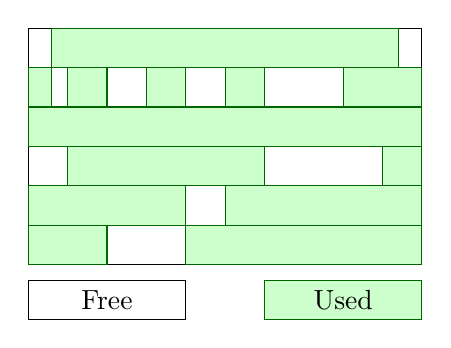
\begin{tikzpicture}
      \draw (0, 0) rectangle (5, 3) ;
      \draw (0, -0.7) rectangle (2, -0.2) node[pos=.5] {Free};
      \filldraw[fill=green!20!white, draw=green!40!black] (3, -0.7) rectangle (5, -0.2) node[pos=.5] {Used};
      \filldraw[fill=green!20!white, draw=green!40!black] (0,0) rectangle (1,0.5);
      \filldraw[fill=green!20!white, draw=green!40!black] (2,0) rectangle (5,0.5);
      \filldraw[fill=green!20!white, draw=green!40!black] (0,0.5) rectangle (2,1);
      \filldraw[fill=green!20!white, draw=green!40!black] (2.5,0.5) rectangle (5,1);
      \filldraw[fill=green!20!white, draw=green!40!black] (0.5,1) rectangle (3,1.5);
      \filldraw[fill=green!20!white, draw=green!40!black] (4.5,1) rectangle (5,1.5);
      \filldraw[fill=green!20!white, draw=green!40!black] (0,1.5) rectangle (5,2);
      \filldraw[fill=green!20!white, draw=green!40!black] (0,2) rectangle (0.3,2.5);
      \filldraw[fill=green!20!white, draw=green!40!black] (0.5,2) rectangle (1,2.5);
      \filldraw[fill=green!20!white, draw=green!40!black] (1.5,2) rectangle (2,2.5);
      \filldraw[fill=green!20!white, draw=green!40!black] (2.5,2) rectangle (3,2.5);
      \filldraw[fill=green!20!white, draw=green!40!black] (4,2) rectangle (5,2.5);
      \filldraw[fill=green!20!white, draw=green!40!black] (0.3,2.5) rectangle (4.7,3);
  \end{tikzpicture}
\end{minipage}

\subsubsection{Grundsätzliches}
\begin{itemize}
  \item Es gibt unterschiedliche Strategien, wie DMM umgesetzt werden kann
  \begin{itemize}
    \item new/delete/malloc/free ist nicht die einzige Variante
  \end{itemize}
  \item Die ''übliche'' Umsetzung mit new/delete beinhaltet die Gefahr der Fragmentierung und dadurch eines nicht deterministischen Verhaltens
  \item Fragmentierung entsteht jedoch nur durch fortlaufendes new/delete
  \item Wenn new nur beim Aufstarten (welches meist nicht zeitkritisch ist) durchgeführt wird, delete erst beim Herunterfahren, dann besteht kein Fragmentierungsproblem
  \item unterschiedliche Konfigurationen können damit sehr elegant gelöst werden
\end{itemize}

\subsubsection{Allocation Strategies}
Each less general than malloc/free/new/delete.
\begin{itemize}
  \item Typically more suited to embedded use.
\end{itemize}
We'll examine:
\begin{itemize}
  \item Fully static allocation.
  \item LIFO allocation.
  \item Pool allocation.
  \item Block allocation.
  \item Region allocation
  \begin{itemize}
    \item An optimization that may be combined with other strategies.
  \end{itemize}
\end{itemize}

\paragraph{Fully Static Allocation}
No heap. Objects are either:
\begin{itemize}
  \item On the stack: Local to a function.
  \item Of static storage duration:
  \begin{itemize}
    \item At global scope.
    \item At namespace scope.
    \item static at file, function, or class scope.
  \end{itemize}
\end{itemize}
Useful when:
\begin{itemize}
  \item Exact or minimum number of objects in system statically determinable.
\end{itemize}

''Allocation'' occurs at build time. Hence:\\
\begin{tabular}{|l|p{7cm}|}
  \hline
  Speed: & essentially infinite; deterministic.\\
  External Fragmentation: & impossible.\\
  Memory leaks: & impossible.\\
  Memory exhaustion: & impossible.\\
  But: & Initialization of static objects in different translation units (TUs) indeterminate.\\
  \hline
\end{tabular}

\paragraph{''Heap Allocation''}
Two common meanings:
\begin{itemize}
  \item Dynamic allocation outside the runtime stack.
  \item \textit{Irregular} dynamic allocation outside the runtime stack.
  \begin{itemize}
    \item Unpredictable numbers of objects.
    \item Unpredictable object sizes.
    \item Unpredictable object lifetimes.
  \end{itemize}
\end{itemize}
We'll use the first meaning.
\begin{itemize}
  \item The second one is just the most general (i.e., hardest) case of the first.
\end{itemize}
User-controlled non-heap memory for multiple variable-sized objects entails heap management:
\begin{lstlisting}[language=C++]
uint8_t buffer[someSize]; // this is basically a heap; create/destroy multiple
// ...                    // different-sized objects in buffer
\end{lstlisting}

\paragraph{The C++ Memory Management Framework}
User-defined memory management typically built upon:
\begin{itemize}
  \item User-defined versions of malloc/free
  \item User-defined versions of operator new/new[], operator delete/delete[]
  \item new handlers:
  \begin{itemize}
    \item Functions called when operator new/new[] can't satisfy a request.
  \end{itemize}
\end{itemize}
Here we focus on allocation strategies suitable for embedded systems.\\

\textbf{Example: LIFO Heap Allocation}\\
\includegraphics[width=0.7\linewidth]{images/AdvancedCPP/lifo}

\begin{lstlisting}[language=C++]
class LIFOAllocator {
public:
  LIFOAllocator(uint8_t* heapAddr, std::size_t heapSize)
    : heapBase(heapAddr), heapEnd(heapAddr+heapSize), heapTop(heapAddr)
  {}
  void* allocate(std::size_t sz) throw (std::bad_alloc);  // not shown
  void deallocate(void* ptr, std::size_t sz) throw ();    // ditto
private:
  uint8_t* const heapBase;
  uint8_t* const heapEnd;
  uint8_t* heapTop;
};
\end{lstlisting}
\begin{itemize}
  \item allocat/deallocate behave like class-specific new/delete.
  \item Pointer data member $\rightarrow$ copying functions should be declared.
  \item If LIFOAllocator templatized, ctor params could be template params.
  \begin{itemize}
    \item The Memory-mapped-IO section has an example.
  \end{itemize}
\end{itemize}

Classes can easily build custom new/delete using LIFOAllocator:
\begin{lstlisting}[language=C++]
uint8_t heapSpace[heapSpaceSize];           // memory for heap
LIFOAllocator customAllocator(heapSpace,    // typically at global scope
                              heapSpaceSize);

void* Widget::operator new(std::size_t bytes) throw (std::bad_alloc)
{
  return customAllocator.allocate(bytes);
}

void Widget::operator delete(void* ptr, std::size_t size) throw ()
{
  customAllocator.deallocate(ptr, size);
}
\end{lstlisting}

\begin{tabular}{|l|p{7cm}|}
  \hline
  Speed: & extremely fast; deterministic. (Assuming you don't run out of memory)\\
  External Fragmentation: & possible, but easy to detect.\\
  Memory leaks: & possible, easy to detect.\\
  Memory exhaustion: & possible.\\
  \hline
\end{tabular}

\paragraph{Pool Allocation}
Heap allocations are all the same size.
\begin{itemize}
  \item Typically because all heap objects are one size.
  \begin{itemize}
    \item Well-suited for class-specific allocators.
  \end{itemize}
  \item Can also work when all heap objects are nearly the same size.
  \begin{itemize}
    \item Then all allocations are the size of the largest objects.
  \end{itemize}
\end{itemize}

Basic approach:
\begin{itemize}
  \item Treat heap memory as an array.
  \begin{itemize}
    \item Each element is the size of an allocation unit, therefore no need to store the size of each allocation.
  \end{itemize}
  \item Unallocated elements are kept on a \textit{free} list.
  \item Allocation/deallocation is a simple list operation:
  \begin{itemize}
    \item Removing/adding to the front of the free list.
  \end{itemize}
\end{itemize}

\begin{lstlisting}[language=C++]
template<std::size_t elementSize>
class PoolAllocator {
public:
  PoolAllocator(uint8_t* heapAddr, std::size_t heapSize);
  void* allocate(std::size_t sz) throw (std::bad_alloc);
  void deallocate(void* ptr, std::size_t sz) throw ();
private:
  union Node {                 // pool element
    uint8_t data[elementSize]; // when in use
    Node* next;                // on free list
  };
  Node* freeList;
};
\end{lstlisting}
\begin{itemize}
  \item Pointer data member $\rightarrow$ copying functions should be declared
  \item If PoolAllocator untemplatized, template param could be ctor param.
  \item Ideally,, we'd ensure that elementSize $>$ 0, better: $\geq$ sizeof(Node*).
\end{itemize}

\textbf{PoolAllocator::PoolAllocator():}
\begin{lstlisting}[language=C++]
template<std::size_t elementSize>
PoolAllocator<elementSize>::PoolAllocator(uint8_t* heapAddr,
                                          std::size_t heapSize)
  : freeList(reinterpret_cast<Node*>(heapAddr))
{
  const std::size_t nElems = heapSize / sizeof(Node);
  for (std::size_t i = 0; i < nElems-1; ++i)    // link array elements
    freeList[i].next = &freeList[i+1];
  freeList[nElems-1].next = nullptr;            // nullptr from and after C++11
}
\end{lstlisting}
\includegraphics[width=0.7\linewidth]{images/AdvancedCPP/poolAllocatorConstructor}

\textbf{PoolAllocator::allocate():}
\begin{lstlisting}[language=C++]
template<std::size_t elementSize>
void* PoolAllocator<elementSize>::allocate(std::size_t bytes) throw (std::bad_alloc)
{
  if (bytes != elementSize)
    return ::operator new(bytes);
  if (freeList != mullptr)
  {
    void* pMem = freeList;        // alignment?
    freeList = freeList->next;
    return pMem;
  }
  else
    throw std::bad_alloc();
}
\end{lstlisting}
\begin{minipage}{0.6\linewidth}
Variation: allow bytes $\leq$ elementSize, i.e., that the request fits.
\begin{itemize}
  \item More flexible, but can lead to internal fragmentation.
\end{itemize}
\end{minipage}
\begin{minipage}{0.4\linewidth}
  \includegraphics[width=\linewidth]{images/AdvancedCPP/internalFragmentation.png}
\end{minipage}

\textbf{PoolAllocator::deallocate():}
\begin{lstlisting}[language=C++]
template<std::size_t elementSize>
void PoolAllocator<elementSize>::deallocate(void* ptr,
                                            std::size_t size) throw ()
{
  if (ptr == nullptr)
    return;
  if (size != elementSize)
  {
    ::operator delete(ptr);
    return;
  }
  Node* p = static_cast<Node*>(ptr);
  p->next = freeList;
  freeList = p;
  ptr = nullptr;  // increases safety
}
\end{lstlisting}

\begin{tabular}{|l|p{7cm}|}
  \hline
  Speed: & extremely fast; deterministic. (Assuming you don't run out of memory and no wrong-sized requests)\\
  External Fragmentation: & impossible.\\
  Memory leaks: & possible.\\
  Memory exhaustion: & possible.\\
  \hline
\end{tabular}

\paragraph{Block Allocation}
Essentially a set of pools with different element (block) sizes:
\includegraphics[width=0.5\linewidth]{images/AdvancedCPP/blockAllocation}
n-byte requests handled by first pool with size $\geq$ n and non-full free list.\\
Useful when:
\begin{itemize}
  \item Allocations needed for a relatively small number of object sizes.
  \begin{itemize}
    \item Otherwise internal fragmentation $\rightarrow$ wasted memory.
  \end{itemize}
\end{itemize}
Many RTOSes offer native support for block allocation.

\begin{tabular}{|l|p{7cm}|}
  \hline
  Speed: & fast; nearly deterministic (and boundable). (Assuming you don't run out of memory and no requests larger than handled by the largest-chunk pool). Speed isn't totally deterministic, because you may need to examine multiple pools to find one with sufficient free memory.\\
  External Fragmentation: & impossible.\\
  Memory leaks: & possible.\\
  Memory exhaustion: & possible.\\
  \hline
\end{tabular}

\paragraph{General Variable-Sized Allocation}
What new/delete/malloc/free already do.
\begin{itemize}
  \item Desirable only if vendor-supplied routines unacceptable.
\end{itemize}
Possible motivations:
\begin{itemize}
  \item Detect overruns/underruns.
  \item Gather heap usage data.
  \begin{itemize}
    \item Size and lifetime distributions, temporal usage patterns, etc.
  \end{itemize}
  \item Support data structre clustering.
  \item Avoid thread-safety penalty.
  \begin{itemize}
    \item ST applications.
    \item Thread-local allocators in MT applications.
  \end{itemize}
\end{itemize}

\paragraph{Region Allocation}
An optimization for when memory for all of a heap's objects can be released at once.
\begin{itemize}
  \item Clients call a region member function at the appropriate time.
  \begin{itemize}
    \item Faster than deallocating each object's memory individually.
  \end{itemize}
  \item Common with LIFO allocators, but compatible with pools, blocks, etc.
  \item operator delete for individual objects a no-op, hence very fast.
  \begin{itemize}
    \item Can still use delete operator to invoke destructors:\\
    \begin{lstlisting}[language=C++]
    delete p;  // invoke *p's dtor, then operator delete on p;
               // if *p in a region, operator delete is a no-op
    \end{lstlisting}
  \end{itemize}
\end{itemize}

\subsubsection{Summary}
\begin{itemize}
  \item Many embedded systems include dynamic memory management.
  \item Key issues are speed, fragmentation, leaks, and memory exhaustion.
  \item LIFO is fast and w/o fragmentation, but object lifetimes must be LIFO.
  \item Pools are fast and w/o fragmentation, but object sizes are limited.
  \item Block allocation is essentially multiple pool allocators.
  \item Regions excel when all heap objects can be released simultaneously.
\end{itemize}


\subsection{C++ and ROMability}
Anything can be burned into ROM and loaded into RAM prior to program execution.
The more interesting question is:
\begin{itemize}
  \item What may remain in ROM as the program runs?
\end{itemize}
The C++ standard is silent on ROMing:
\begin{itemize}
  \item It allows essentially anything, guarantess nothing.
  \item What's ROMable is thus up to your compiler and linker.
\end{itemize}
In what follows, we disucss what is \textit{technically possible}.
\begin{itemize}
  \item Your compiler/linker probably imposes some restrictions.
\end{itemize}

\subsubsection{C++ and ROM}
To understand the restrictions, we need to know what a ''POD type'' is.
\begin{itemize}
  \item All C data types are POD (Plain Old Data) types.
  \item C++11 classes, structs, and unions are generally POD types if they lack:
  \begin{itemize}
    \item Base classes
    \item Virtual functions
    \item Non-static data members of reference type
    \item User-defined constructors, destructor, or assignment operators
    \item Non-static data members of non-POD types
  \end{itemize}
\end{itemize}
Essentially, a C++11 class or struct is a POD type if it's ''laid out like C and its semantics are preserved if it's memcpyed.''
\begin{itemize}
  \item But note that non-virtual member functions are allowed.
  \item Static data and static member functions are allowed, too.
\end{itemize}

Common restrictions on ROMing data:
\begin{itemize}
  \item Many compilers/linkers will ROM only statically initialized POD types.
  \begin{itemize}
    \item As we'll see, it is technically possible for some dynamically initialized non-PODs to be ROMed.
  \end{itemize}
  \item Some compilers/linkers woll ROM structs, but not classes.
  \begin{itemize}
    \item There is no technical reason for this distinction.
  \end{itemize}
  \item By the way: ROM is slower than RAM (but RAM is more expensive)
\end{itemize}

Program instructions can always be ROMed.
Data in C++ program can be ROMed if it meets two criteria:
\begin{itemize}
  \item Its value is known before runtime.
  \begin{itemize}
    \item i.e., either the compiler or the linker knows it or can compute it.
  \end{itemize}
  \item It can't be modified at runtime.
\end{itemize}

Examples:
\begin{lstlisting}[language=C++]
static const int table[] = {1, 2, 3};    // table is ROMable

const char* pc1 = "Hello World";         // "Hello World" is ROMable
                                         // (but pc1 is not)

const char* const pc2 = "World";         // "World" is ROMable (and may be
                                         // shared with "Hello World"
                                         // pc2 is also ROMable
\end{lstlisting}

\paragraph{TI: Const types}
Hidden Cost
\begin{itemize}
  \item Global const variables in C may be allocated to SRAM and have their init value in flash.
  \item In all cases, the value would normally be loaded from memory (unless the compiler can see its initial value).
  \item Static const scalar variables are like \lstinline{#define} macro constants and will not be stored in memory if not needed (address not taken, value small enough to be an immediate).
\end{itemize}

Cortex-M3
\begin{itemize}
  \item Different compilers and optimization levels will affect how global const is treated.
  \item Static const is more reliable for all compilers.
  \item Enum constants are also a good choice (and can be used with normal ints).
\end{itemize}

\subsubsection{C++ und ROM: int-Konstanten}
\begin{itemize}
  \item Explizit vorhandene int-Konstanten im Sourcecode sollten wegoptimiert werden. Im Normalfall ergibt eine int-Konstante eine Immediate-Adressierung (MOVE \#123, R1)
  \item 3 Möglichkeiten für die Definition
  \begin{itemize}
    \item const int
    \begin{compactitem}
      \item gute Möglichkeit
      \item wenn Adresse genommen wird, kann die Konstante nicht wegoptimiert werden
      \item u.U. mehrere Kopien im Code
    \end{compactitem}
    \item enum
    \begin{compactitem}
      \item allerbeste Möglichkeit
      \item sollte ausschliesslich verwendet werden
      \item (negative Werte sind auch möglich)
    \end{compactitem}
    \item \#define
    \begin{compactitem}
      \item keine Vorteile ggü. anderen Methoden
      \item kein Scope
      \item können nicht private oder protected sein
    \end{compactitem}
  \end{itemize}
\end{itemize}

\subsubsection{C++ und ROM: double-Konstanten}
\begin{itemize}
  \item double-Konstanten können kaum wegoptimiert werden (Immediate-Adressierung geht normalerweise nicht)
  \item Ausnahme: bei 64 Bit-Systemen kann es gehen oder bei guter FPU
  \item 2 Möglichkeiten für die Definition
  \begin{itemize}
    \item const double
    \begin{compactitem}
      \item gute Möglichkeit
    \end{compactitem}
    \item \#define
    \begin{compactitem}
      \item Makroproblematik
      \item private, protected nicht möglich
      \item häufig mehrere Kopien dieser Konstanten im Code
    \end{compactitem}
  \end{itemize}
\end{itemize}

\subsubsection{C++ and ROM: Objects}
\begin{itemize}
  \item Objects may be ROMed if the following are true:
  \begin{itemize}
    \item They are declared const at their point of definition.
    \item They contain no mutable data members.
    \item They are initialized with values known during compilation.
    \begin{itemize}
      \item Such ''knowledge'' might come from dataflow analysis, etc.
    \end{itemize}
  \end{itemize}
\end{itemize}
\begin{lstlisting}[language=C++]
struct Point
{
  int x;
  int y;
};

const Point origin = {0, 0};  // origin is ROMable
\end{lstlisting}

\subsubsection{C++ and ROM: Compiler Generated Data}
Some compiler generated data structures can usually be ROMed:
\begin{itemize}
  \item Virtual function tables
  \item RTTI (RunTime Type Information) tables and type\_info objects
  \item Tables supporting exception handling
\end{itemize}
ROMing these objects may be impossible if they are dynamically linked from shared libraries.

\subsubsection{Summary: C++ and ROM}
\begin{itemize}
  \item Most compilers/linkers are willing to ROM statically initialized POD types.
  \begin{itemize}
    \item Aggressive build chains may go beyond this.
  \end{itemize}
  \item ROMable PODs can be encapsulated by making them protected or private in a non-POD type.
  \item Compiler-generated data structures are typically ROMable.
\end{itemize}


\subsection{Modeling Memory Mapped IO (MMIO)}
Many subsystems map IO devices to fixed parts of a program's address space.
\begin{itemize}
  \item Input registers are often separate from output registers.
  \item Control/status registers are often separate from data registers.
  \begin{itemize}
    \item Different status register bits convey information such as readiness or whether device interrupts are enabled.
  \end{itemize}
\end{itemize}
C++ makes it easy to make memory-mapped IO devices look like objects with natural interfaces.
\begin{itemize}
  \item \textbf{At zero cost.}
  \begin{itemize}
    \item Provided you have a decent compiler :-)
  \end{itemize}
\end{itemize}

Memory-mapped devices may require special handling, e.g.,
\begin{itemize}
  \item Atomic reads/writes may require explicit synchronization.
  \item Individual bits may sometimes be read-only, other times write-only.
  \item Clearing a bit may require assigning a 1 to it (positive vs. negative logic).
  \item One control register may control more than one data register.
  \begin{itemize}
    \item E.g., bits 0-3 are for one data register, bits 4-7 for another.
  \end{itemize}
\end{itemize}
What follows is a \textit{framework} for modeling memory-mapped IO, not a prescription.
\begin{itemize}
  \item The framework tells you where to put whatever special handling your devices require.
  \item It's an elegant and efficient way to define a HAL.
\end{itemize}

\subsubsection{Grundsätzliches zu MMIO}
(siehe HAL in EmbSW1)
\begin{itemize}
  \item Embedded Systems werden sehr intensiv mittels Registern programmier, d.h. durch Setzen oder Löschen einzelner Bits
  \item Register können mittels Bitfeldern modelliert werden.
  \begin{itemize}
    \item Nicht portabel
    \item Können sehr ineffizient sein (manchmal aber auch sehr effizient)
    \item Erlauben nur sehr eingeschränkte Abstraktion
    \item Sollten generell vermieden werden
  \end{itemize}
  \item Register müssen auf eine bestimmte Adresse gemappt werden können
  \item MMIO Register \textbf{müssen} mit \textbf{volatile} gekennzeichnet werden
\end{itemize}

\subsubsection{Modeling a Control Register}
Suppose we have a fout-byte control register such that:
\begin{itemize}
  \item Bit 0 indicates readiness: 1 $\rightarrow$ ready, 0 $\rightarrow$ not ready.
  \item Bit 2 indicates whether interrupts are enabled: 1 $\rightarrow$ enabled, 0 $\rightarrow$ not.
\end{itemize}
\begin{lstlisting}[language=C++]
enum {bit0 = 0x1, bit1 = 0x2, ... , bit31 = 0x80000000};
class ControlReg {
public:
	bool ready() const {return (regValue & bit0) == bit0;}
	bool interruptsEnabled() const {return (regValue & bit2) == bit2;}
	void enableInterrupts() {regValue |= bit2;}
	void disableInterrupts() {regValue &= ~bit2;}
private:
	volatile uint32_t regValue;		// register data may change outside program control
};
\end{lstlisting}

Notes:
\begin{itemize}
  \item All functions are inline, so their existence should incur no cost.
  \item enableInterrupts() and disableInterrupts() use read/modify/write instructions, so they may be subject to race conditions in multithreaded systems.
  \item We assume that the register is both readable and writable.
  \begin{itemize}
    \item If it's write-only, you'll need to cache the most recently written value.
  \end{itemize}
\end{itemize}

\subsubsection{Placement new}
\begin{itemize}
  \item Die Aufgabe des Operators new ist nicht primär, Speicher zu allozieren, sondern eine Adresse zurückzugeben auf einen bestimmten Speicherbereich.
  \item Üblicherweise wird new zusammen mit dem Allozieren von Speicher verwendet.
  \item \textbf{Placement new} ist eine Variante des new-Operators, die ein Objekt an eine bestimmte Stelle im Speicher legt. Eine Speicherallozierung ist damit nicht verbunden.
  \item Ein durch placement new platziertes Objekt muss und darf nicht mit delete gelöscht werden!
\end{itemize}

\paragraph{Place a Register at Address Using Placement mew}
\begin{lstlisting}[language=C++]
// create a ControlReg object at address 0xFFFF0000 and make pcr point to it
ControlReg* const pcr = new (reinterpret_cast<void*>(0xFFFF0000)) ControlReg;

// avoid pointer syntax
ControlReg& cr = *new (reinterpret_cast<void*>(0xFFFF0000)) ControlReg;

while (!cr.ready())               // wait until the ready bit is on
{}
cr.enableInterrupts();            // enable device interrupts
if (cr.interruptsEnabled()) ...   // if interrupts are enabled
\end{lstlisting}

\paragraph{Placement new vs. Raw Casts}
Our use of placement new calls the default ControlReg constructor.
\begin{itemize}
  \item It's implicit, inline, and empty.
  \begin{itemize}
    \item It should optimize away (i.e., to zero instructions).
    \item \textbf{If it doesn't and you care} (or if your compiler doesn't support placement new), consider a reinterpret\_cast instead of placement new:
  \end{itemize}
\end{itemize}
\begin{lstlisting}[language=C++]
// pointer version
ControlReg* const pcr = reinterpret_cast<ControlReg*>(0xFFFF0000);

// reference version
ControlReg& cr = *reinterpret_cast<ControlReg*>(0xFFFF0000);
\end{lstlisting}
\textbf{Placement new is typically preferable to a raw reinterpret\_cast}:
\begin{itemize}
  \item It works if the device object's constructor has work to do.
  \item A raw cast will behave improperly in that case.
\end{itemize}
But there are times when reinterpret\_cast can be superior:
\begin{itemize}
  \item If placement new isn't optimized to zweo instructions (and you care).
  \item If you want to ROM the address of an IO register \textit{and}
  \begin{itemize}
    \item Your compiler will ROM the result of a reinterpret\_cast \textit{and}
    \item It won't ROM the result of a use of placement new.
  \end{itemize}
\end{itemize}

\subsubsection{Placing Objects via Compiler Extensions}
With some compilers/linkers, there is another alternative:
\begin{itemize}
  \item Use a compiler extension to place an object at a specific address.
\end{itemize}
Examples:
\begin{itemize}
  \item Altium Tasking compilers offer this kind of syntax:\\
  \lstinline[language=C++]{ControlReg cr __at(0xFFFF0000);}
  \item The Wind River Diab compiler offers this:\\
  \begin{lstlisting}[language=C++]
  #pragma section MMIO address=0xFFFF0000
  #pragma use_section MMIO cr
  ControlReg cr;
  \end{lstlisting}
\end{itemize}
Such extensions may impose restrictions:
\begin{itemize}
  \item E.g., such manually-placed objects may have to be POD types.
  \item It's not portable.
\end{itemize}
Payoffs:
\begin{itemize}
  \item No need to access MMIO objects indirectly through a pointer.
  \item No need to allocate space for a pointer to each MMIO object.
\end{itemize}

\subsubsection{Placing Objects via Linker Commands}
Linkers may support specification of where objects are to be placed:
\begin{itemize}
  \item C++ source code is ''normal''.
  \begin{itemize}
    \item No object placement information is present.\\
    \lstinline[language=C++]{ControlReg cr;}
  \end{itemize}
  \item Linker scripts map C++ objects to memory locations, often by:
  \begin{itemize}
    \item Mapping objects to sections.
    \begin{itemize}
      \item The linker sees only \textit{mangled} names.
    \end{itemize}
    \item Mapping sections to address ranges.
  \end{itemize}
\end{itemize}
Result is more portable C++ code.
\begin{itemize}
  \item Platform-specific addresses mentioned only in linker scripts.
\end{itemize}

\subsubsection{Modeling an Output Device, Take 1}
An uint32\_t-sized output device register can be modeled as a ControlReg object bundled with the uint32\_t-sized data it controls:
\begin{lstlisting}[language=C++]
class OutputDevice1
{
public:
  OutputDevice1(uint32_t controlAddr,
                uint32_t dataAddr);
  ControlReg& control() {return *pcr;}      // get ControlReg
  void write(uint32_t value) {*pd = value;} // write data to device
private:
  ControlReg* const pcr;                    // ptr to ControlReg; note const
  volatile uint32_t* const pd;              // ptr to data; note const and volatile
};
\end{lstlisting}

The constructor makes pcr and pd point to the correct addresses:
\begin{lstlisting}[language=C++]
OutputDevice1::OutputDevice1(uint32_t controlAddr,
                             uint32_t dataAddr)
  : pcr(new (reinterpret_cast<void*>(controlAddr)) ControlReg),
    pd(new (reinterpret_cast<void*>(dataAddr)) uint32_t)
{}
\end{lstlisting}

Clients use the class like this:
\begin{lstlisting}[language=C++]
OutputDevice1 od(0xFFFF0000,     // ctrl reg addr
                 oxFFFF0004);    // data reg addr
uint32_t x;
// ...
while (!od.control().ready())   // wait until the ready bit is on
{}
od.write(x);                    // write x to od
// ...
\end{lstlisting}

\subsubsection{Modeling an Output Device, Take 2}
MMIO addresses are compile-time constants, so it shouldn't be necessary to store them as data members like pcr and pd.\\
A template with non-type parameters makes it easy not to:
\begin{lstlisting}[language=C++]
template<uint32_t controlAddr, uint32_t dataAddr>
class OutputDevice2
{
public:
                                                // ctor now gone
  static ControlReg& control()
  {return *reinterpret_cast<ControlReg*>(controlAddr);}
  static void write(uint32_t value)
  {*reinterpret_cast<volatile uint32_t*>(dataAddr) = value;}
                                                // data members now gone
};
\end{lstlisting}
OutputDevice2 uses static member functions to avoid passing \textit{this} pointers.

This example assumes the ControlReg constructor/destructor do nothing.
\begin{itemize}
  \item Otherwise OutputDevice2 will need a constructor/destructor that call them (e.g., via placement new).
\end{itemize}
\begin{lstlisting}[language=C++]
template<uint32_t controlAddr, uint32_t dataAddr>
class OutputDevice2
{
public:
  OutputDevice2()
  {new (reinterpret_cast<ControlReg*>(controlAddr)) ControlReg;}
  // ...
};
\end{lstlisting}
\textbf{Such initialization/cleanup must occur only once!}
\begin{itemize}
  \item Problematic if multiple OutputDevice2 objects exist for a single hardware device.
  \begin{itemize}
    \item Use Singleton to prevent multiple instantiations?
    \item Use static alreadyInitialized/alreadyCleanedup flags?
  \end{itemize}
\end{itemize}


Client code looks almost the same as before:
\begin{lstlisting}[language=C++]
OutputDevice2<0xFFFF0000, 0xFFFF0004> od;
uint32_t x;
// ...
while (!od.control().ready())  // wait until the ready bit is on
{}
od.write(x);                   // write x to od
// ...
\end{lstlisting}
Advantages of this approach:
\begin{itemize}
  \item OutputDevice2 objects are smaller than OutputDevice1 objects.
  \item OutputDevice2 code may also be smaller/faster than OutputDevice1 code.
  \begin{itemize}
    \item No need to go indirect via a this pointer.
  \end{itemize}
\end{itemize}

\subsubsection{Modeling an Output Device, Take 3}
\textit{If}, as in this case, the \textbf{control and data registers are in contiguous memory}, you can use a third design:
\begin{itemize}
  \item Create objects \textit{directly} on the MMIO locations:
\end{itemize}
\begin{lstlisting}[language=C++]
class OutputDevice3
{
public:
  ControlReg& control() {return cr;}
  void write(uint32_t value) {data = value;}
private:
  OutputDevice3(const OutputDevice3&);  // prevent copying
  ControlReg cr;
  volatile uint32_t data;
};
\end{lstlisting}
\begin{itemize}
  \item Have clients use placement new (or bare reinterpret\_cast) themselves:
\end{itemize}
\begin{lstlisting}[language=C++]
// create OutputDevice3 object at address 0xFFFF0000
OutputDevice3& od = *new (reinterpret_cast<void*>(0xFFFF0000)) OutputDevice3;
\end{lstlisting}

\subsubsection{Modeling Hardware Directly}
There are thus two kinds of classes for modeling memory-mapped IO.\\
One kind models hardware \textit{directly}.
\begin{itemize}
  \item Objects of such classes are created by clients at specific addresses.
  \begin{itemize}
    \item Via placement new or reinterpret\_cast.
  \end{itemize}
  \item They contain only non-static data that maps to MMIO registers:
\end{itemize}
\begin{lstlisting}[language=C++]
class OutputDevice3
{                       // class designed to be instantiated at MMIO addresses
public:
  // ...
private:
  OutputDevice3(const OutputDevice3&);
  ControlReg cr;        // data members map directly to MMIO device registers
  volatile uint32_t data;
};
\end{lstlisting}
\begin{itemize}
  \item Static data is okay.
  \item They never contain virtual functions (virtual functions leads to a vptr \textit{somewhere} within each object).
\end{itemize}

\subsubsection{Modeling Hardware Indirectly}
The other kind models hardware \textit{indirectly}.
\begin{itemize}
  \item Objects of such classes are \textbf{not} created at specific addresses.
  \begin{itemize}
    \item Clients pass MMIO addresses as template of constructor arguments.
  \end{itemize}
  \item They may contain ''extra'' data members.
  \begin{itemize}
    \item i.e., that don't correspond to MMIO device registers.
  \end{itemize}
\end{itemize}
\begin{lstlisting}[language=C++]
class OutputDevice1
{
// ...
private:
  ControlReg* const pcr;        // data members that don't map
  volatile uint32_t* const pd;  // to MMIO device registers
  uint32_t lastValueWritten;    // useful for write-only regs
};
\end{lstlisting}

They may contain virtual functions:
\begin{lstlisting}[language=C++]
class DeviceBase {
public:
  virtual void reset() = 0;
  // ...
};
class OutputDevice1: public DeviceBase {
public:
  void reset() override;
  // ...
};
template<uint32_t controlAddr, uint32_t dataAddr>
class OutputDevice2: public DeviceBase {
public:
  void reset() override;
  // ...
};
OutputDevice1 od1a(0xFFFF0000, 0xFFFF0004);
OutputDevice1 od1b(0xFFFF0010, 0xFFFF0014);
// ...
OutputDevice2<0xEEEE0000, 0xEEEE0010> od2a;
OutputDevice2<0xEEEE0020, 0xEEEE0040> od2b;
// ...
DeviceBase* registers[] = {&od1a, &od1b, ..., &od2a, &od2b, ...};
const std::size_t numRegisters = sizeof(registers)/sizeof(registers[0]);
// ...
for (std::size_t i = 0; i < numRegisters; ++i)
{                       // reset all registers in system
  registers[i]->reset();
}
\end{lstlisting}

\textbf{Indirect modeling more expensive than direct modeling}:
\begin{itemize}
  \item Memory for ''extra'' data members (if present).
  \item Indirection to get from the object to the register(s) (if needed).
\end{itemize}
It's also more flexible:
\begin{itemize}
  \item May add other data members.
  \item May declare virtual functions.
\end{itemize}


\subsubsection{Preventing Likely Client Errors}
Clients that model hardware directly can easily be misused, e.g.:
\begin{itemize}
  \item Clients might instantiate them at non-MMIO addresses.
  \item Clients who use placement new might think they need to call delete.
  \begin{itemize}
    \item They don't, though they may need to manually call the destructor.
  \end{itemize}
\end{itemize}
\textbf{To prevent such errors, consider declaring the destructor private.}


\begin{tabular}{|p{9.2cm}|p{9.2cm}|}
\begin{lstlisting}
class OutputDevice3    // class modeling hardware directly
{                      // prevents some kinds of client errors
  // ...
private:
  ~OutputDevice3() {}
  ControlReg cr;
  volatile uint32_t data;
};
\end{lstlisting}
&
\begin{lstlisting}
OutputDevice3 d;  // error! implicit destructor invocation. (We want to preven
                  // MMIO objects from being placed on the stack.)

OutputDevice3* pd =
  new (reinterpret_cast<void*>(0xFFFF0000)) OutputDevice3; // fine
// ...
delete pd;        // error! another implicit destructor invocation
\end{lstlisting}
\end{tabular}

\paragraph{Basic idea:}
\textbf{A fundamental design goal is that \textit{design violations} should not compile.}

\subsubsection{Generalizing via Templates}
Devices are likely to vary in several ways:
\begin{itemize}
  \item Number of bits in each register.
  \item Which bits correspond to ready and interrupt status, etc.
\end{itemize}
Templates make it easy to handle such variability:
\begin{lstlisting}[language=C++]
template<typename RegType, RegType readyBitMask, RegType interruptBitMask>
class ControlReg {
public:
  bool ready() const {
    return (regValue & readyBitMask) == readyBitMask;}
  bool interruptsEnabled() const {
    return (regValue & interruptBitMask) == interruptBitMask;}
  void enableInterrupts() {regValue |= interruptBitMask;}
  void disableInterrupts() {regValue &= ~interruptBitMask;}
private:
  volatile RegType regValue;
};
\end{lstlisting}

\paragraph{Usage}
\begin{lstlisting}[language=C++]
// CRui03 is a control register the size of an uint32_t where
// bit 0 is the ready bit and bit 3 is the interrupt bit

typedef ControLReg<uint32_t, bit0, bit3> CRui03;

CRui03& cr1 = *new (reinterpret_cast<void*>(0xFFFF0000)) CRui03;
// ...    // use cr1


// CRuc15 is a control register the size of an uint8_t where
// bit 1 is the ready bit and bit 5 is the interrupt bit

typedef ControLReg<uint8_t, bit1, bit5> CRuc15;

CRuc15& cr2 = *new (reinterpret_cast<void*>(0xFFFF0010)) CRuc15;
// ...    // use cr2
\end{lstlisting}

\subsubsection{Summary}
C++ tools you'll probably want to use:
\begin{itemize}
  \item Classes
  \item Class templates (with both type and non-type parameters)
  \item Inline functions
  \item Placement new and reinterpret\_cast
  \item const pointers
  \item volatile memory
  \item References
  \item Private member functions, e.g., copy constructor, destructor.
\end{itemize}
